\newpage
\thispagestyle{sectioned}
\chapter{Arquitectura del Proyecto}

\section{Arquitectura de Wave}

    \subsection{Modelo Wave}\label{sec:waveModel}
    
    Además de definir el protocolo del que hace uso Wave, Google definió un Modelo de Datos Conversacional \cite{ref:wave_conversation_model} que refleja la arquitectura de los datos que componen las conversaciones en Wave. Así, a grandes rasgos, podemos ver dichas conversaciones como documentos XML sobre los que los usuarios participantes (cualquiera es libre de unirse a una conversación en cualquier momento) actúan creando nuevos elementos o modificando los ya existentes. Este modelo de datos define una nomenclatura propia para los elementos que componen esta tecnología \cite{ref:wave_api_overview} \cite{ref:wave_white_paper}:
    
      \begin{itemize}
	\item \textbf{Wave}: Conjunto de wavelets (conversaciones).
	\item \textbf{Wavelet}: conjunto de documentos de una conversación y sus participantes.
	\item \textbf{Blip}: documento con el contenido de un mensaje en la conversación. Un blip puede tener otros blips dentro de él y los blips pueden ser publicados o no en función de si su visibilidad se extiende o no al resto de participantes de la conversación respectivamente.
	\item \textbf{Manifiesto conversacional}: documento con metadatos que definen la estructura de una conversación. 
	\item \textbf{Hilo conversacional}: conjunto de Blips consecutivos que forman parte de una conversación.
	\item \textbf{Extensiones} \cite{ref:wave_extensions}: pequeñas aplicaciones que se ejecutan dentro de una Wave y aportan nuevas funcionalidades que no forman parte del modelo conversacional básico. Pueden ser de dos tipos:
	  \begin{itemize}
	    \item \textbf{Gadget}: aplicación que se ejecuta en el contexto de una Wave y en la que todos sus usuarios participan.
	    \item \textbf{Robot}: aplicación que participa en una Wave a modo de usuario automatizado e interactúa con el contenido pudiendo modificarlo y responder a eventos por acciones de otros usuarios reales.
	  \end{itemize}
      \end{itemize}
      
       \begin{figure}[H]
	  \centering
	    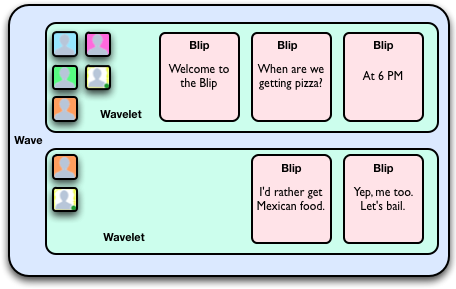
\includegraphics[keepaspectratio, scale=0.8]{Media/Captures/waveEntities.png}
	  \caption{Modelo Conversacional de Wave}
	  \label{fig:wave_model}
	\end{figure}
	
	\subsection{Modelo SwellRT}

\section{Arquitectura de la aplicación}

La arquitectura está compuesta por cuatro módulos principales de los que hablaremos en profundidad en las siguientes subsecciones. Como \textbf{Cliente móvil} tendremos la aplicación desarrollada en Android, que realizará peticiones HTTP al servicio web alojado en OpenShift \cite{ref:OpenShift}, una plataforma que permite alojar servicios web de forma gratuita. Dentro del servicio contaremos con una \textbf{API RESTful} que será quien gestione las peticiones de la aplicación móvil mediante el protocolo HTTP.

CAMBIAR FOTO PARA VER INTEGRACION CON WAVE

\begin{figure}[H]
\centering
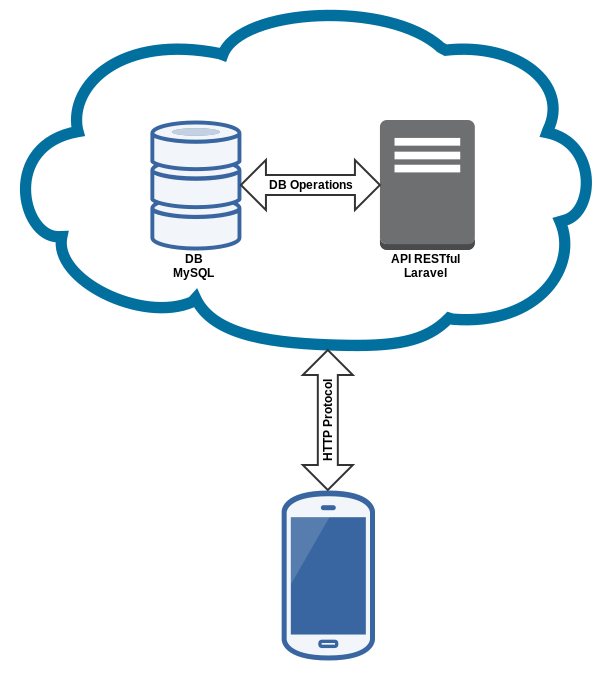
\includegraphics[keepaspectratio, scale=0.4]{Media/Captures/architecture.png}
\caption{Arquitectura de la aplicacción.}
\label{fig:architecture}
\end{figure}

Por otro lado, la aplicación hará uso del \textbf{Servicio Android} desarrollado en SwellRT-Android \cite{ref:swellRT_android_github} para conectarse con el servidor Wave alojado en https://wave.p2pvalue.eu/ e intercambiar los datos que sea necesario mantener en tiempo real, es decir, la edición de una Propuesta de forma colaborativa entre varias personas.

Por último, la \textbf{Base de Datos MySQL} alojada en el servidor de OpenShift almacenará toda la información relacionada con la aplicación. La API RESTful será quien actúe de intermediario entre las peticiones de la aplicación y las operaciones en Base de Datos.

\subsection{Base de datos}

En la implementación de la Base de Datos se ha utilizado un Modelo Relacional para la definición de las tablas. Utilizando MySQL \cite{ref:MySQL} como sistema de gestión de base de datos (SGBD) y phpMyAdmin \cite{ref:phpMyAdmin} como herramienta de gestión gráfica de la base de datos.

La base de datos está formada por un total de 12 tablas donde se almacena toda la información relacionada con los programas de los partidos políticos, las propuestas ciudadanas, encuestas, comparativas... y otros datos más técnicos como la gestión de los usuarios, la relación de los comentarios o la relación entre las secciones y comparativas entre otras.

\begin{figure}[H]
\centering
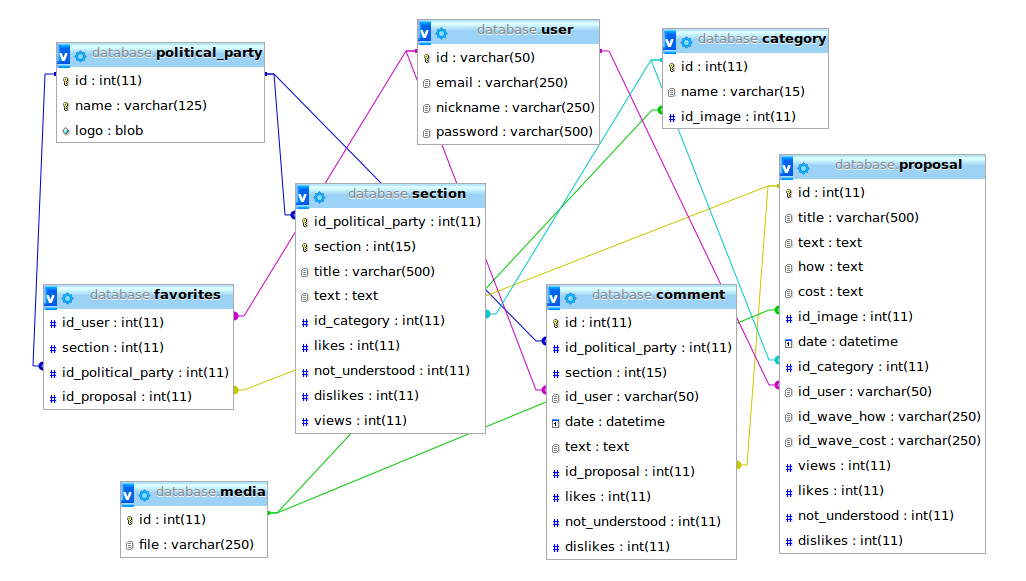
\includegraphics[keepaspectratio, scale=0.30]{Media/Captures/database.png}
\caption{Modelo entidad-relación de la base de datos.}
\label{fig:ermodel}
\end{figure}

Las tablas \textit{section} y \textit{political-party} son utilizadas para guardar información estática en la aplicación. Es decir, en la tabla \textit{political-party} se almacenan los partidos políticos que se presentan a unas elecciones, y en la tabla \textit{section}, las diferentes secciones de un programa electoral. Tan sólo modificaremos las columnas de \textit{likes}, \textit{dislikes}, \textit{not-understood} y \textit{views} para obtener estadísticas de uso de cada sección. El resto de las columnas permanecerán intactas.

EXPLICAR RESTO DE TABLAS. DATOS ESTATICOS VS DINAMICOS

Las demás tablas serán utilizadas para guardar datos dinámicos de la aplicación. Datos que normalmente genera un usuario visitando una sección de un programa, creando una propuesta, haciendo un comentario, etc.

\subsection{Service REST}

Para establecer la conexión de la aplicación desarrollada en Android con la Base de Datos hemos utilizado \textbf{Laravel} como Servicio Web. Laravel \cite{ref:laravel} es un framework de código abierto para desarrollar aplicaciones web con PHP 5. Laravel permite además montar una API REST (Representational State Transfer), un estilo de arquitectura software para sistemas hipermedia distribuidos como la World Wide Web. Este término se originó en una tesis doctoral sobre la web escrita por Roy Fielding \cite{ref:RESTPhd}. La elección de Laravel como framework PHP fue debida a su flexibilidad, la facilidad para programar la aplicación y el gran soporte que tiene de la comunidad. Además Laravel cuenta con una licencia de software libre MIT, lo que nos permite continuar utilizando software en todo el proyecto, y fue el Framework más popular al finales de 2013.

\begin{figure}[H]
\centering
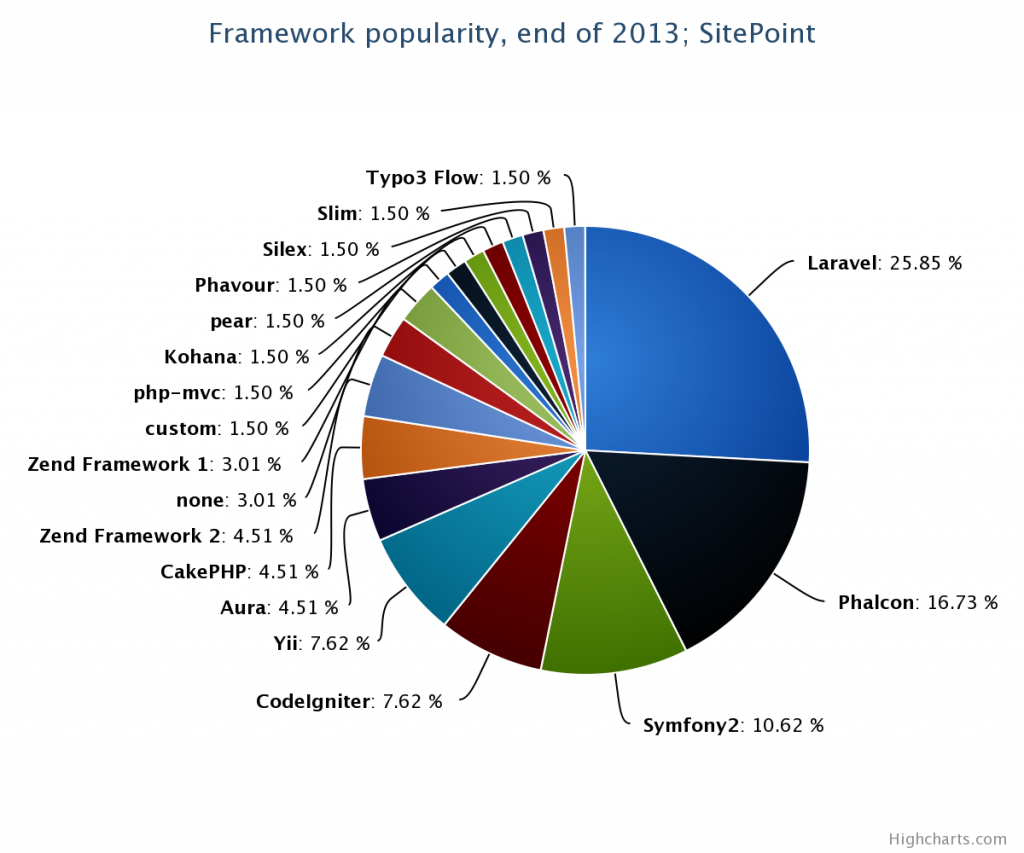
\includegraphics[keepaspectratio, scale=0.30]{Media/Captures/frameworkPopularity.png}
\caption{Pantalla principal de Laravel 5.}
\label{fig:laravel5}
\end{figure}

Laravel nos permite implementar un sistema RESTful para que el cliente móvil pueda hacer peticiones al servicio web y que dicho servicio responda a éstas de la forma que queramos. Estas peticiones se realizan mediante el protocolo HTTP. En función de la operación que deseemos hacer, clasificaremos estas funciones en el acrónimo \textbf{CRUD} \cite{ref:CRUD} (del original en inglés: \textbf{C}reate, \textbf{R}ead, \textbf{U}pdate and \textbf{D}elete).

\begin{table}[H]
\begin{tabular}{|c|c|c|m{6.25cm}|}
\hline
{\bf Petición} & {\bf Operación} & {\bf SQL} & \multicolumn{1}{c|}{{\bf Utilidad}}              \\ \hline
GET            & Leer            & SELECT    & Obtener un recurso almacenado en el servidor.    \\ \hline
POST           & Crear           & INSERT    & Crear un nuevo recurso en el servidor.           \\ \hline
PUT            & Actualizar      & UPDATE    & Actualizar un recurso almacenado en el servidor. \\ \hline
DELETE         & Borrar          & DELETE    & Eliminar un recurso almacenado en el servidor.   \\ \hline
\end{tabular}
\caption{Funciones CRUD}
\label{fig:CRUDtable}
\end{table}

En función de las peticiones que realicemos al servicio que serán realizadas mediante el protocolo HTTP, el servidor nos devolverá un código de estado para obtener el \textit{feedback} de lo sucedido. Por tanto distinguiremos diferentes códigos de estado cuando queramos obtener un recurso, actualizar un recurso, crear uno nuevo o borrarlo. En la siguiente tabla se definen los códigos de estado que puede devolvernos el servidor en función de nuestras peticiones.

\begin{table}[H]
\begin{tabular}{|c|c|m{7.5cm}|}
\hline
{\bf Petición} & {\bf Status Code} & \multicolumn{1}{c|}{{\bf Descripción}}                         \\ \hline
GET            & 200 (OK)          & El recurso solicitado ha sido devuelto correctamente.          \\ \hline
GET            & 404 (Not Found)   & El recurso solicitado no ha sido encontrado.                   \\ \hline
POST           & 201 (Created)     & El nuevo recurso ha sido creado correctamente.                 \\ \hline
POST           & 404 (Not Found)   & No se ha especificado el nuevo recurso a crear.                \\ \hline
POST           & 409 (Conflict)    & No se ha podido crear el recurso porque ya existe.             \\ \hline
PUT            & 200 (OK)          & El recurso ha sido actualizado correctamente.                  \\ \hline
PUT            & 204 (No Content)  & No se ha especificado el recurso que pretende ser actualizado. \\ \hline
PUT            & 404 (Not Found)   & El recurso a actualizar no ha sido encontrado.                 \\ \hline
DELETE         & 200 (OK)          & El recurso solicitado ha sido borrado.                         \\ \hline
DELETE         & 404 (Not Found)   & El recurso solicitado para borrar, no ha sido encontrado.      \\ \hline
\end{tabular}
\caption{Códigos de estado de la respuesta del servidor}
\label{fig:codeStateRestTable}
\end{table}

Usar un servicio RESTful nos proporciona una gran flexibilidad a la hora de independizar la tecnología del servidor de la del cliente. Mediante la arquitectura basada en peticiones HTTP no solo podremos hacer peticiones desde el cliente en Android, sino que más adelante podriamos desarrollar una versión web o incluso un cliente para iOS sin tener que modificar el servicio, ya que las peticiones HTTP serán las mismas.

\subsubsection{Arquitectura}

Laravel utiliza implementa un funcionamiento basado en el patrón \textbf{MVC} (Model–view–controller), separando el modelo de la vista, y delegando la gestión al controlador. En nuestro caso tendríamos un modelo almacenado en las tablas de la base datos, donde se guardará toda la información dinámica y estática de la aplicación. El controlador sería en elcargado de gestionar las peticiones del cliente en Android en función del tipo de operación que requiera. Y por último, tendríamos como vista el resultado devuelto por el servidor con los datos solicitados por el cliente, que a su vez los representaría en la aplicación móvil. Esta estructura de comportamiento hace independiente el modelo controlado por el servidor, de la vista que obtiene el usuario final en su cliente móvil. Con esto conseguimos eleborar un código más claro y sencillo, así como también evitar conflictos entre el modelo y la vista.

\begin{figure}[H]
\centering
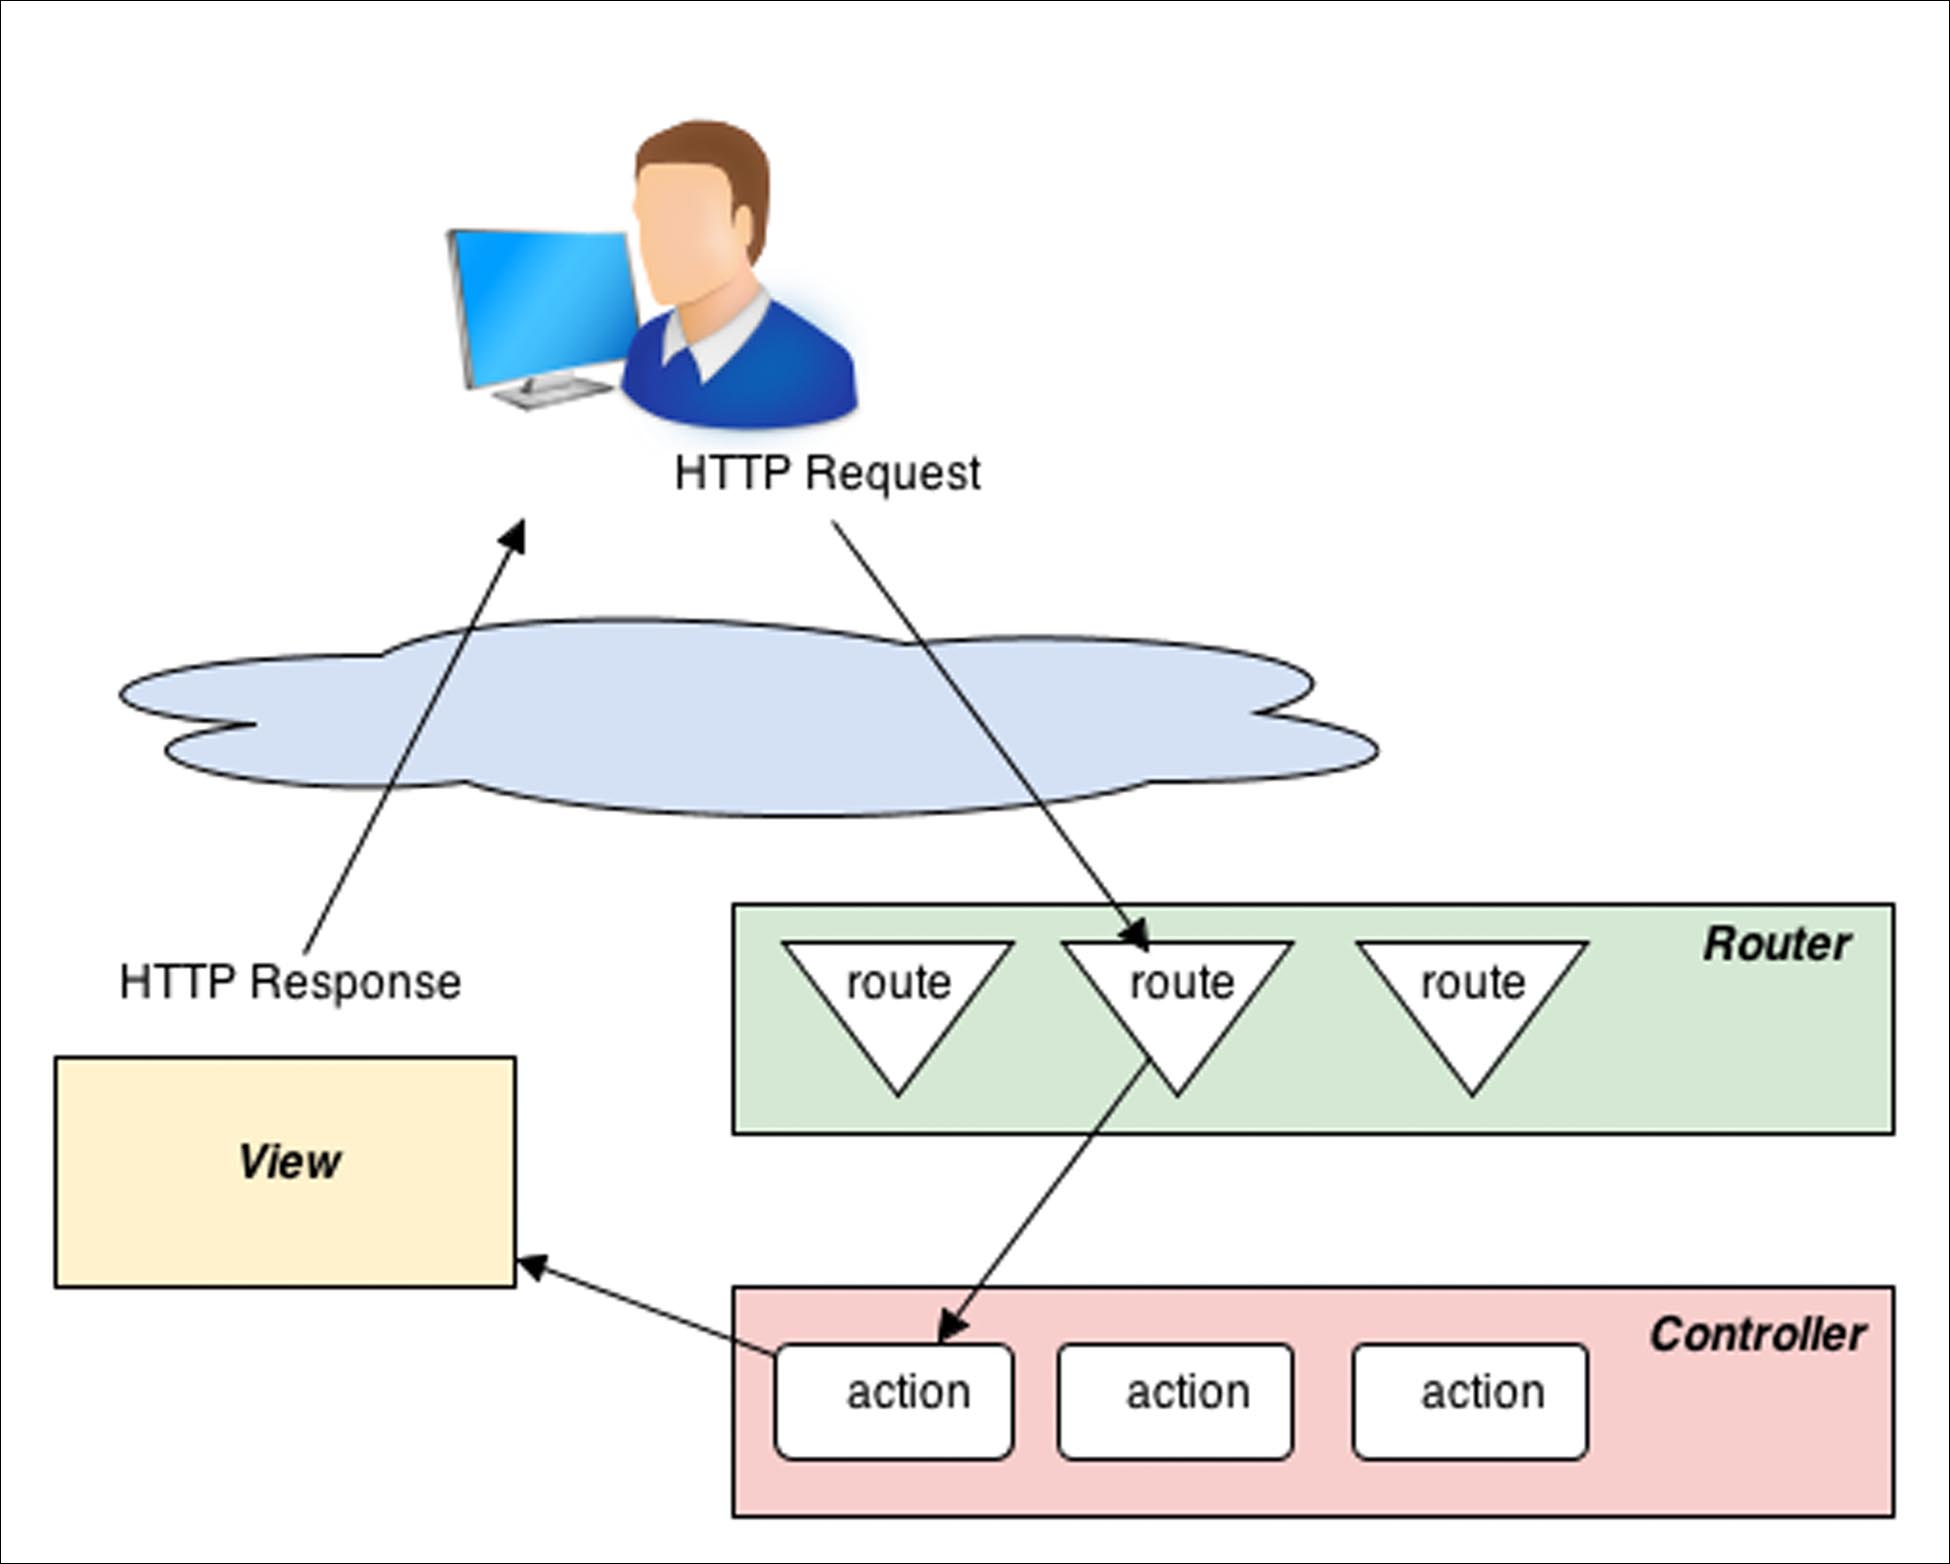
\includegraphics[keepaspectratio, scale=0.8]{Media/Captures/laravelArch.jpg}
\caption{Arquitectura de Laravel}
\label{fig:laravelArch}
\end{figure}

Para comprender la arquitectura de Laravel vamos a destacar tres componentes clave. En primer lugar tenemos una primera capa que gestiona las peticiones del cliente. Esta capa estará compuesta por una serie de \textbf{rutas} a las que el cliente realizará la petición en función de la operación que quiera realizar. Después, en función de la ruta que haya realizado la petición, se adentrará en una nueva capa compuesta por \textbf{controladores} que se encargarán de procesar la petición y devolver al cliente lo que ha solicitado. Éste último componente será la \textbf{vista}, que puede ser representada de muchas formas. En nuestro caso, la vista estará compuesta en una serie de datos en formato JSON, que posteriormente el cliente móvil se encargará de representar la vista. Visto esto, procederemos a detallar un poco más estos tres componentes fundamentales.

\subsubsection{Rutas}

Cómo citábamos en anteriormente, la primera capa de Laravel es un \textit{mapa de rutas} que definirá todos los caminos posibles para llegar a la funcionalidad requerida de los controladores. Todas las rutas estarán definidas en el fichero \textbf{routes.php}, alojado en la carpeta \textit{app/Http/routes.php} de nuestra instalación Laravel. El archivo \textit{routes.php} es un fichero muy simple escrito en PHP donde definiremos todas las rutas posibles. La definición de una ruta irá acompañada de tres valores. El primero de ellos será el tipo de petición que realizará el cliente (ver tabla \ref{fig:CRUDtable}), seguido de la definición de la url por la que será accesible, y por último, indicaremos el controlador responsable de procesar la petición. A parte de indicar el controlador, también hay que indicar el método que procesará la petición dentro del controlador como veremos más adelante.

Para definir el conjunto de urls que forman el archivo \textit{routes.php}, hemos seguido una serie de buenas prácticas \cite{ref:practicesRESTful_API} habituales a la hora de desarrollar una RESTful API. Normalmente utilizaremos nombres en lugar de verbos para acceder a los resursos. Por ejemplo, si queremos visualizar el listado de propuestas de la aplicación, utilizaremos la url \textit{/proposal}. Que será definida como:	

\lstset{
   language        = php}
\begin{lstlisting}[frame=single]	
Route::get('/proposal', 'ProposalController@index');
\end{lstlisting}

Así queda definida la ruta que accede a todo el listado de propuestas como una petición GET, que se encargará de procesarla el controlador \textit{ProposalController} en su método \textit{index()}.

Para acceder a una propuesta en concreto, se pasará un \textit{id} para obtener el recurso adecuado. Este \textit{id} irá a continuación de la url anteriormente definida. Por ejemplo, si quisiéramos acceder a la propuesta cuyo id es igual a 5, definiríamos la siguiente ruta:

\lstset{
  language        = php}
  \begin{lstlisting}[frame=single]	
Route::get('/proposal/{id}', 'ProposalController@show');
\end{lstlisting}

Nótese  ruta es la misma que la anterior, a la que hemos añadido un nuevo parámetro que deberá especificar el usuario. Así la petición \textit{GET /proposal/5}, nos devolvería la propuesta con id 5. Si nos fijamos, el controlador también es el mismo, pero esta vez el método encargado de procesar la petición será \textit{show()}. Además este método recibirá el parámetro \textit{{id}} que envíe el usuario en la petición.

Para crear una nueva propuesta en la aplicación, deberemos realizar una petición POST. Nuestra ruta será exactamente igual que la primera, pero antes deberemos especificar que se trata de una ruta que atenderá a una petición POST:

\lstset{
  language        = php}
\begin{lstlisting}[frame=single]	
Route::post('/proposal', 'ProposalController@create');
\end{lstlisting}

Donde una vez más en controlador \textit{ProposalController} se encargará de procesar la petición en el método \textit{create}. Si nos fijamos en la primera ruta dónde obteníamos las propuestas (\textit{GET /proposal}, es exactamente igual que la que acabamos de definir. Sólo les diferencia el tipo de petición que está realizando el cliente. Para definir otros tipos de peticiones como PUT o DELETE, usaremos la misma metodología. El resultado final de las peticiones que podrían realizarse a una propuesta quedería definida de la siguiente forma:

\lstset{
  language        = php}
\begin{lstlisting}[frame=single]
// Posibles operaciones con el objeto "propuesta"
Route::get('/proposal', 'ProposalController@index');
  // Obtiene el listado de todas las propuestas
Route::get('/proposal/{id}', 'ProposalController@show');
  // Obtiene la prupuesta pasada por el campo {id}
Route::post('/proposal', 'ProposalController@create');
  // Crea una nueva propuesta en el servidor
Route::put('/proposal/{id}', 'ProposalController@update');
  // Actualiza la propuesta pasada por {id}
Route::delete('/proposal/{id}',
			    'ProposalController@destroy');
  // Borra la propuesta pasada por {id}
\end{lstlisting}

Para organizar el código y poder visualizarlo de forma clara utilzaremos grupos de rutas. Esto nos resultará especialmente útil cuando tengamos varias operaciones que realizar dentro de una misma dirección, definiendo una nueva ruta cuya función será definida a continuación, incluyendo las rutas que vienen dentro del grupo. Si nos fijamos en el ejemplo anterior, podemos observar como todas las url comienzan con \textit{/proposal}. Por ello no es necesario definir en cada línea la ruta \textit{/proposal}, si no que bastará con definirla en un único grupo que adjuntará todas las rutas que comienzen de la misma forma. Así nuestro ejemplo anterior quedaría más claro y ordenado de la siguiente forma:

\lstset{
  language        = php}
\begin{lstlisting}[frame=single]
Route::group(['prefix' => 'proposal'], function()
{
    Route::get('/', 'ProposalController@index');
    Route::get('/{id}', 'ProposalController@show');
    Route::post('/', 'ProposalController@create');
    Route::put('/{id}', 'ProposalController@update');
    Route::delete('/{id}','ProposalController@destroy');
});
\end{lstlisting}

De esta forma podemos visualizar de un vistazo todas las posibilidades agrupadas dentro de la dirección \textit{proposal}. Lo que nos permitirá utilizar grupos para ordenar funciones comunes dentro de un mismo prefijo, y además crear subgrupos dentro de los anteriores si tenemos algún prefijo repetido varias veces. Esto podría aplicarse a nuestro ejemplo anterior, agrupando las peticiones que requieren como parámetro un \textit{id} de la propuesta:

\lstset{
  language        = php}
\begin{lstlisting}[frame=single]
Route::group(['prefix' => 'proposal'], function()
{
  Route::get('/', 'ProposalController@index');
  Route::post('/', 'ProposalController@create');
  Route::group(['prefix' => '/{id}'], function()
  {
    Route::get('/', 'ProposalController@show');
    Route::put('/', 'ProposalController@update');
    Route::delete('/','ProposalController@destroy');
  });
});
\end{lstlisting}

HACE FALTA ALGO MÁS...?

\subsubsection{Controladores}

Los controladores son los encargados de procesar todas las operaciones que intervienen en el modelo, es decir, en la información almacenada en la base de datos. Un controlador es un fichero escrito en PHP que será almacenado en la ruta \textit{/app/Http/Controllers} de la aplicación. Este fichero estará formado por una métodos y atributos que serán llamados desde las rutas definidas en la aplicación. Cada controlador hereda de una clase abstracta llamada \textit{Controller}, que a su vez esta hereda de la clase abstracta \textit{BaseController}. La cual implementa la funcionalidad básica de los controladores.

\begin{figure}[H]
\centering
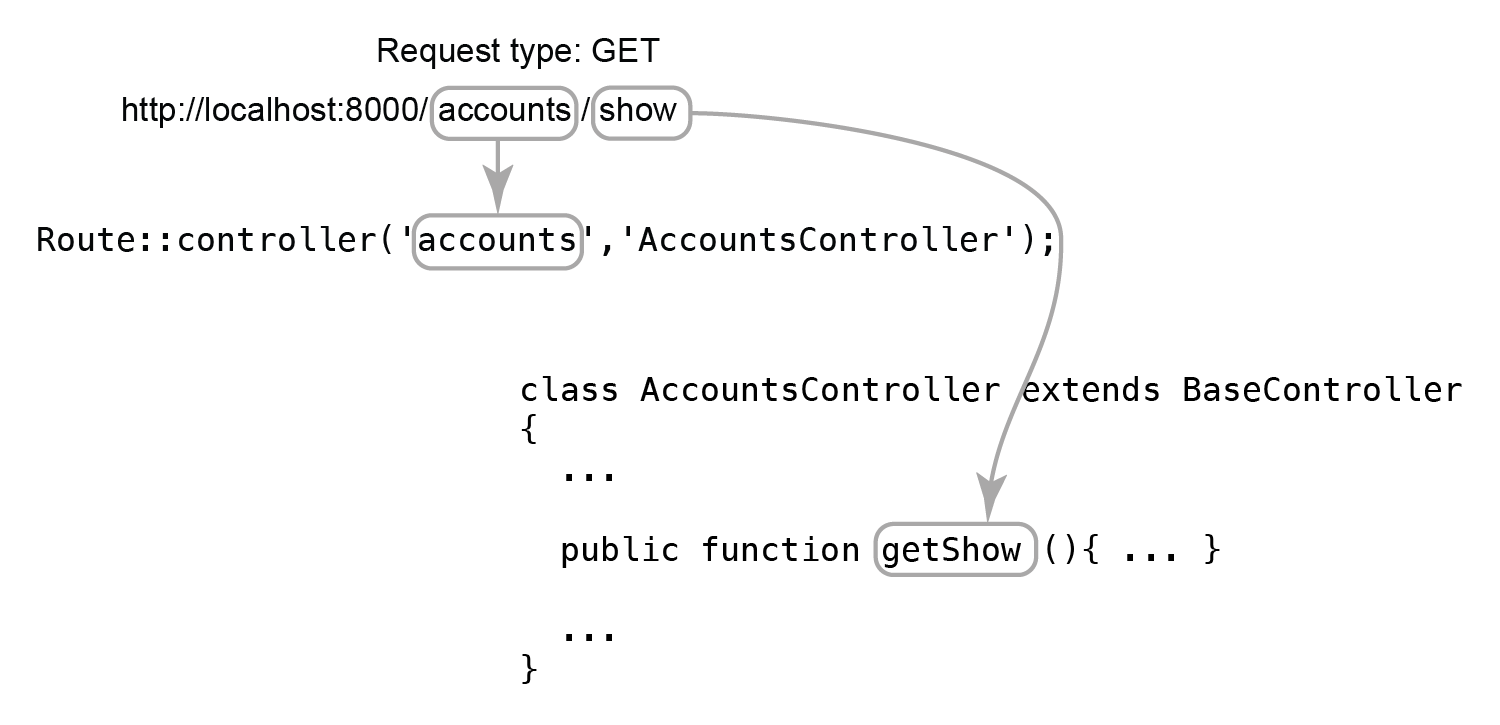
\includegraphics[keepaspectratio, scale=1]{Media/Captures/getDiagramMethod.png}
\caption{Camino desde la ruta al método del controlador.}
\label{fig:laravelArch}
\end{figure}

Dentro de un controlador definiremos aquellos métodos que correspondan con las rutas de la aplicación. Estos métodos procesarán la información del cliente, operando con los parámetros que haya obtenido, accediendo a la base de datos, y devolviendo una respuesta en función del éxito de la operación. El siguiente ejemplo muestra una implementación básica del método \textit{index()} del \textit{ProposalController}:

\lstset{
  language        = php}
\begin{lstlisting}[frame=single]
<?php namespace App\Http\Controllers;

use App\Http\Requests;
use App\Http\Controllers\Controller;
use DB;

class ProposalController extends Controller {
  /**
  * Display a listing of the resource.
  *
  * @return Response
  */
  public function index()
  {
    return DB::select('SELECT * FROM `proposal`');
  }
}
\end{lstlisting}

La conexión a la base de datos se encuentra configurada en el archivo \textit{/config/database.php}, por lo que la gestión de la conexión y desconexión será controlada por Laravel. Lo que nos proporciona más independencia y versatilidad a la hora de programar. Como respuesta del método, Laravel utiliza por defecto un fichero JSON con los resultados de la variable a la que asigenmos el resultado, o a la sentencia SQL de la consulta que estemos devolviendo. El siguiente ejemplo muestra cuál sería el resultado de realizar una petición GET a la dirección \textit{/proposal}:

\lstset{
  language        = c,    inputencoding=utf8}
\begin{lstlisting}[frame=single]
[
  {"id":1,"title":"Reducir la contaminaci\u00f3n en Madrid","text":"Actualmente la contaminaci\u00f3n en Madrid est\u00e1 llegando a unos l\u00edmites por encima de la media de las principales ciudades de la Uni\u00f3n Europea. Por ello deber\u00edamos reducir esa contaminaci\u00f3n ambiental acerc\u00e1ndonos a la media europea.","how":"Cerrando el tr\u00e1fico en determinadas zonas de Madrid. Distrito: Zona Centro.","cost":"Hacer 7 km de calles peatonales: 750.000 \u20ac","id_image":4,"date":"2015-05-06 00:00:00","id_category":4,"id_user":"6d823fa54c6d1a12","views":4,"likes":3,"not_understood":0,"dislikes":0},
  {"id":2,"title":"Restaurar el plan de estudios del '98","text":" Lorem ipsum dolor sit amet, consectetur adipiscing elit. Praesent lobortis, sapien eget dignissim efficitur, augue eros molestie purus, et gravida erat quam a lacus. Fusce vel eros cursus, venenatis dui ac, aliquet risus. Fusce euismod ex at varius lacinia. Sed at urna condimentum orci volutpat eleifend nec id erat. Sed at vestibulum neque. Maecenas vehicula hendrerit felis, quis condimentum arcu commodo eu. Sed egestas, orci eget ultricies mollis, est leo porttitor sem, at elementum enim arcu ut magna. ","how":"Suprimienndo el plan Bolonia de los grados de 4 a\u00f1os a licenciaturas y diplomaturas.","cost":"Coste 0.","id_image":2,"date":"2015-05-18 00:00:00","id_category":2,"id_user":"d2d115f79ab3a7a4","views":12,"likes":0,"not_understood":1,"dislikes":0}
]
\end{lstlisting}

\subsection{Servicio Android de conexión con Wave}

REORDENAR LO DE WAVE

\subsection{Cliente Android}

INTERFAZ GRAFICA -> PRESENTACION AL USUARIO

ALGORITMO ESTRUCTURACION DE PROGRAMA

ARQUITECTURA DE PETICIONES AL REST

ARQUITECTURA DE PETICIONES A WAVE

